\documentclass[12pt, utf8]{beamer}
\usepackage[ngerman]{babel}
\usepackage{xcolor}
\usepackage{graphicx}
\usepackage {listingsutf8}
\usepackage{multicol}

%AnnArbor | Antibes | Bergen |
% Berkeley | Berlin | Boadilla |
% boxes | CambridgeUS | Copenhagen |
% Darmstadt | default | Dresden |
% Frankfurt | Goettingen |Hannover |
% Ilmenau | JuanLesPins | Luebeck |
% Madrid | Malmoe | Marburg |
% Montpellier | PaloAlto | Pittsburgh |
% Rochester | Singapore | Szeged |
% Warsaw

%Einbinden des Themes
\usetheme{Berlin}
%Standard Angaben
\author{Lucius Bachmann, Fabio Sulzer, Frank Müller, Oliver Wisler}
\title{SwissDefcon}
\date{\today}


\definecolor{dkgreen}{rgb}{0,0.6,0}
\definecolor{gray}{rgb}{0.5,0.5,0.5}
\definecolor{mauve}{rgb}{0.58,0,0.82}


\begin{document}

\begin{frame}
\titlepage
\end{frame}

\begin{frame}[allowframebreaks,allowdisplaybreaks]
\frametitle{Inhaltsverzeichnis}
\setcounter{tocdepth}{1}
\tableofcontents
\end{frame}


\section{Einführung}
\subsection{Spielidee}
\begin{frame}{Spielidee}
\begin{itemize}
\item Verfeindete Kantone bekämpfen sich
\item Dabei stehen verschiedene Waffen und Gebäude zur Verfügung
\item Beschränkt durch das Kantonsbudget
\end{itemize}
\end{frame}

\section{Spielstatus}

\subsection{Spielstatus}
\begin{frame}{Spielstatus}
Was muss gespeichert werden?
\begin{multicols}{2}
\begin{itemize}
\item Spielerdaten
\begin{itemize}
\item Geld
\item Gebiet
\item Objekte
\end{itemize}
\item Objektdaten
\begin{itemize}
\item Standort
\item Lebenspunkte
\end{itemize}
\end{itemize}
\end{multicols}
\end{frame}

\subsection{Verwaltung Spielstatus}

\subsection{Verwaltung mehere Spiele}


\subsection{Clients}

\section{Spielregeln}
\subsection{Welche gibt es?}
\begin{frame}{Spielregeln}
\begin{itemize}
\item
\end{itemize}
\end{frame}


\subsection{Implementation}
\begin{frame}{Implementation}
\begin{figure}
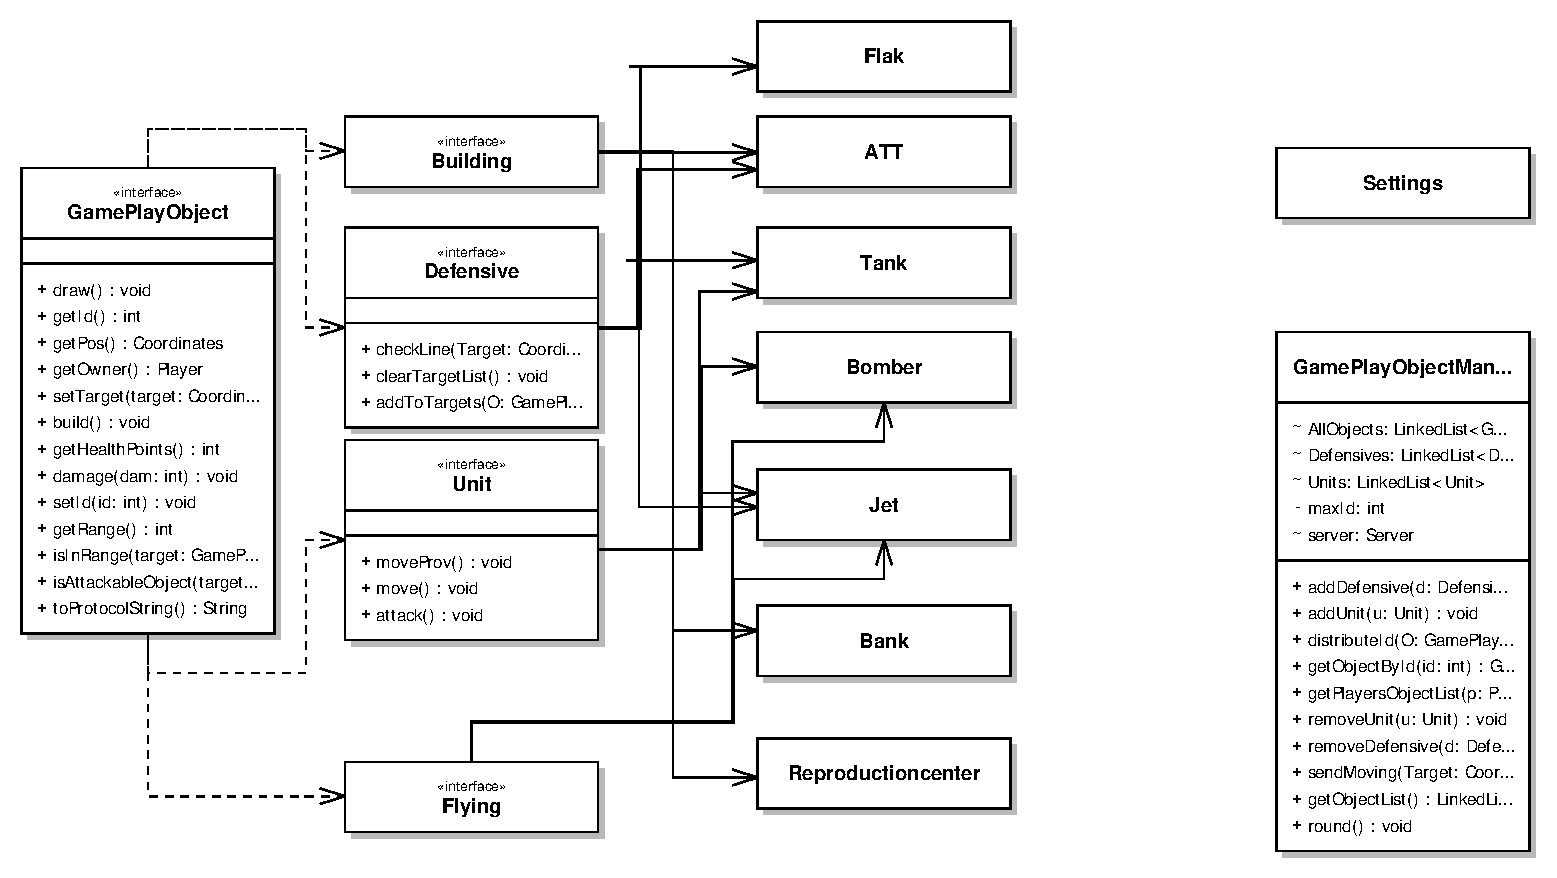
\includegraphics[width=9cm]{images/GamePlayObjects.pdf}
\caption{Klassendiagramm der Spielobjekte}
\end{figure}
\end{frame}


\section{Kommunikation}
\begin{frame}
\subsection{Discovery-Service}

\begin{exampleblock}{Server Broadcast}

\end{exampleblock}
\begin{figure}
\includegraphics[width=6cm]{images/broadcast.eps}
\end{figure}
\end{frame}

\subsection{Chat und Broadcast}
\begin{frame}

\end{frame}
\subsection{Netzwerkprotokoll}
\begin{frame}

\end{frame}

\section{Arbeitsplan}
\subsection{Arbeitsplan}
\begin{frame}
\centering
\includegraphics[scale=0.3]{images/CS108.pdf}
\end{frame}

\subsection{Ist}
\begin{frame}{Ist-Stand}
\begin{itemize}
\item Lobby und Chat fertig
\item Serverstruktur fertig % ???? FRANK
\item bis jetzt geschrieben:
\begin{itemize}
\item 7939 Linien Code
\item 2050 Linien Kommentare
\end{itemize}

\end{itemize}
\end{frame}

\subsection{noch zu tun}
\begin{frame}{to do}
\begin{itemize}
\item Schnittstelle Spiellogik $\leftrightarrow$ Server
\item Schnittstelle Clientparser $\leftrightarrow$ GUI des Spieles
\item Ausbau der GUI
\end{itemize}
\end{frame}

\section{Qualitätssicherung}
\subsection{Ist}
\begin{frame}{QS bis jetzt}
\begin{itemize}
\item eigene Log Klasse und viele Log-Messages
\item gute Dokumentation mit Javadoc
\item viele Kommentare (bis jetzt 20\%)
\item Aufteilung in Pakete nach Funktion
\end{itemize}
\end{frame}

\subsection{noch geplant}
\begin{frame}
Unit Test
-Welche Klasse
\end{frame}


\section{Demo}
\subsection{Demo}
\begin{frame}{Demo}
\begin{itemize}
\item Discovery Service
\item Lobby
\item Chat und private Messaging
\item Spiel erstellen und starten
\item Server Broadcasts
\item evtl. Lucius Simulation Spiellogik
\end{itemize}
\end{frame}

\end{document}